\documentclass[11pt,a4paper]{article}
\usepackage[T1]{fontenc}
\renewcommand{\familydefault}{\sfdefault}
\usepackage{graphicx}
\usepackage{listings}
\usepackage[font=small,labelfont=bf]{caption}
\usepackage[font=scriptsize]{subcaption}
\usepackage{float}
\usepackage{fancyhdr}
\newenvironment{codetext}{\fontfamily{pcr}\selectfont}{\par}


\begin{document}
\begin{titlepage} 
\begin{figure}[H]
  \centering
    
\includegraphics[width=0.3\textwidth]{extra/logo}
\end{figure}
\centering
\rmfamily\Huge\bfseries ~\\~\\~\\~\\  A Tutorial on MD\rmfamily\LARGE\bfseries ~ \\ ~ \\ Probing dynamic effects on protein catalysis
\\~\\~\\ 

\sffamily \Large Erik Marklund\\

\sffamily \Large Joana Filipa Costeira Paulo\\

\sffamily\Large Malin L�king

\sffamily\normalsize ~\\original authors:\\
Fabian Steffen-Munsberg, Paul Bauer and Lynn Kamerlin\\ 

\vfill

\sffamily\large Enzymology and Bioorganic Catalysis\\

Autumn 2017
\end{titlepage}
\clearpage
%\section*{\rmfamily Overview}

\tableofcontents

%This small handbook/tutorial is aimed at giving you an insight about the features and applications of Molecular dynamics (MD) simulations, as well as showing the steps involved in setting up an enzyme system for catalysis and data analysis.
%The system studied here will be the alcohol dehydrogenase A (ADH-A) enzyme from \textit{Rhodococcus rhuber} that you by now should be familiar with after the experimental parts of the course.
%The aim for you will be to set up and perform the initial parts of the dynamics simulation, together with the analysis of a complete data set obtained previously for the same system.
%All the simulations and analysis will be performed using the software GROMACS (http://www.gromacs.com), one of the many programs available to perform full atomistic simulations of biomolecules.
%GROMACS itself is less one single program and more a set of individual parts that allow you to prepare, simulate and subsequently analyse a system.
%For a full overview over everything that is possible, please refer to the official documentation\cite{Abraham2015a}.
%This also contains parts about the theory behind MD that might be useful if you are interested in this kind of studies.

%This tutorial will follow a general outline shown below for each day:\\


%Day one:
%\begin{itemize}
%\item{System background}
%\item{System preparation - PDB file and GRO file}
%\item{System preparation - Solvation and ionisation}
%\item{Protein minimization}
%\item{Protein heating and equilibration\\}
%\end{itemize}


%Day two:
%\begin{itemize}
%\item{Data analysis - Mirror images and artefacts}
%\item{Data analysis - RMSD}
%\item{Data analysis - Distance measurements}
%\item{Data analysis - Clustering of structures\\}
%\end{itemize}


%Day three:
%\begin{itemize}
%\item{Synopsis\\}
%\end{itemize}

%Also, as some of you might not be familiar with the use of UNIX like systems, a small section is included on how to navigate through folders using the command line interface available at the supercomputing center.
%This will also help you in setting up the directory structure needed for the tutorial.\\


%Day Zero:
%\begin{itemize}
%\item{The UNIX shell}
%\item{Creating and removing folders}
%\item{Archives}
%\item{Copying of files and folders\\}
%\end{itemize} 

%At the end of the lab course, you should now have some idea about how to perform and critically analyse simulations using GROMACS.
%The tutorial will be conducted in groups of two, mainly due to the limited amount of computer time available.
%You are still encouraged to try some of the parts on your own while the resources are available, but please consider how much time is needed for any test you might be wanting to simulate.

\clearpage
\section{\rmfamily Day one}
\subsection{\rmfamily System background}
\label{sec:background}
The full atomistic simulation of any protein is a challenging task, even today.
Not so much due to the amount of computer resources needed, but more because it is difficult to set up the simulation in a meaningful way that includes controls and finally allows a physical description of the problem being studied.
In our case here, the problem studied is the difference in binding of the enantiomers of the substrates phenylethanediol and phenylethanol to the enzyme $\cdot$ NAD$^+$ complex.
What is observed is that the enzyme prefers one sterical conformation of the substrate over the other, independent of the fact that it is the alcohol or diol variant.
The binding itself is visualized in Figure \ref{fig:1}, showing you how each of the enantiomeres of a diol substrate might bind to the active site.
\begin{figure}[h]
\center
	\begin{subfigure}[b]{0.45\textwidth}
		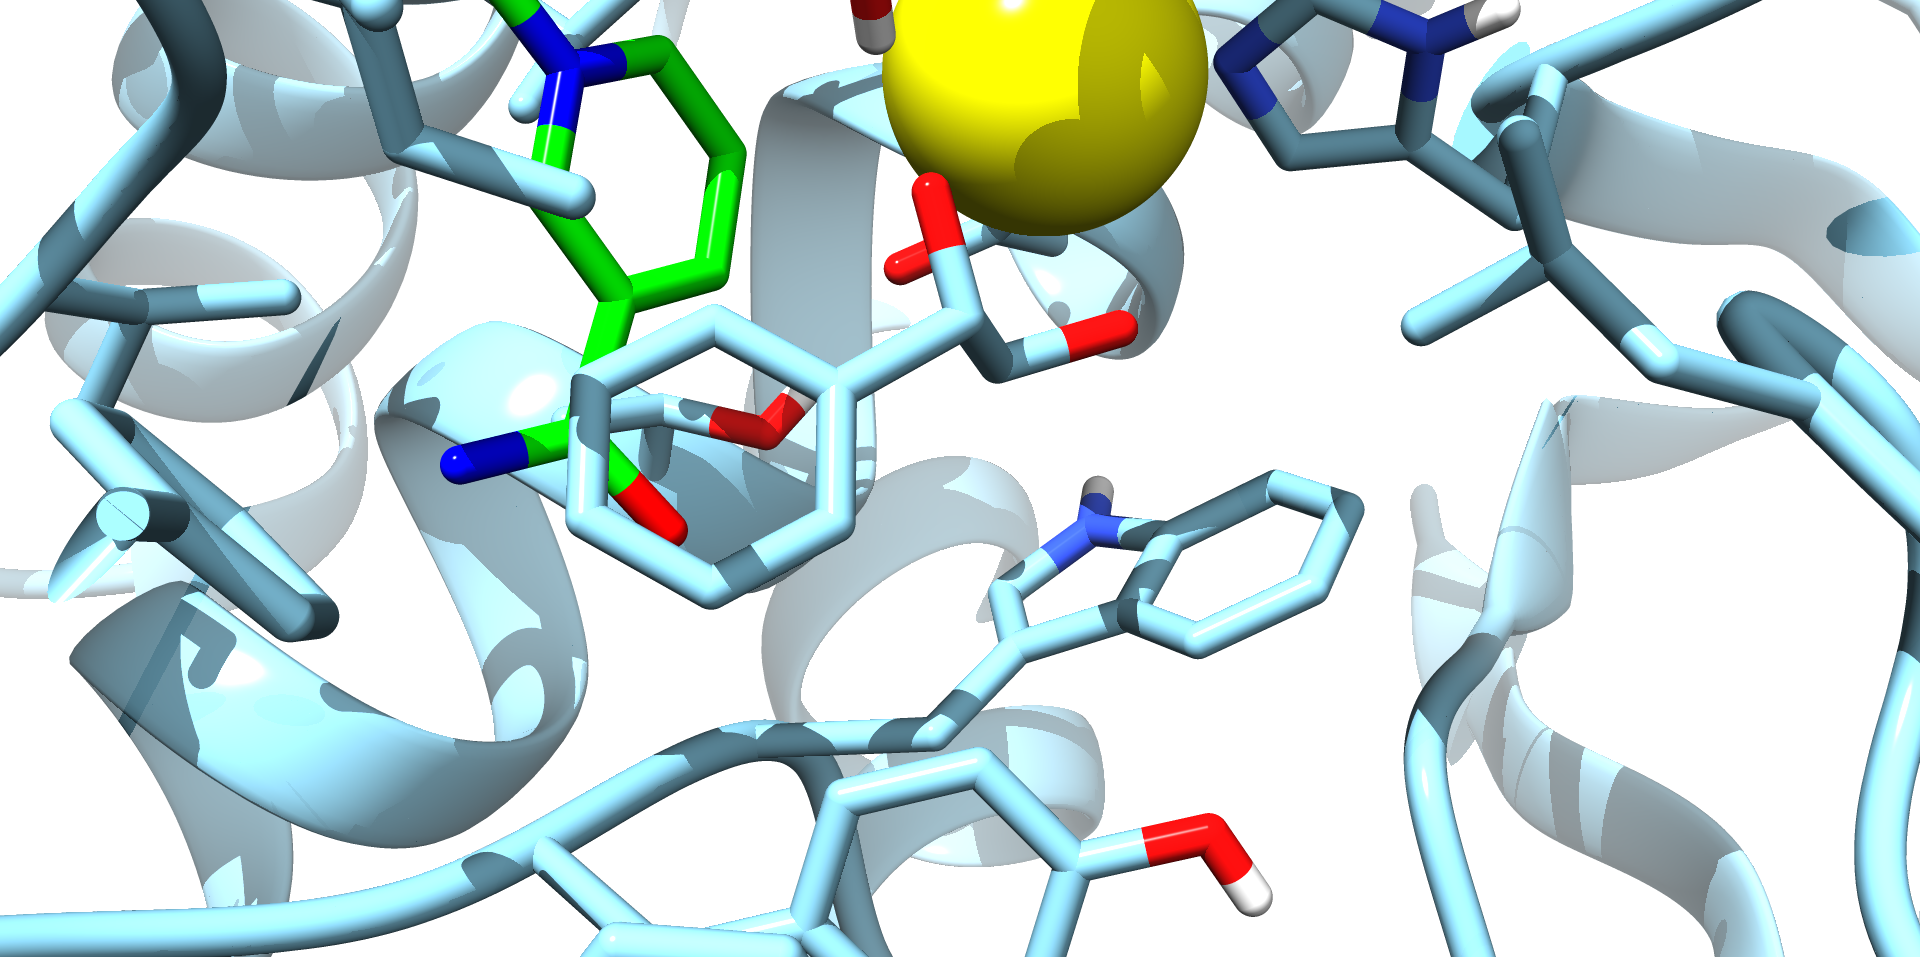
\includegraphics[width=\textwidth,keepaspectratio]{extra/diol-s.png}
		\caption{ADH-A active site with bound S-Phenylethanediol substrate}
		\label{fig:1.1}
	\end{subfigure}
~ 
	\begin{subfigure}[b]{0.45\textwidth}
		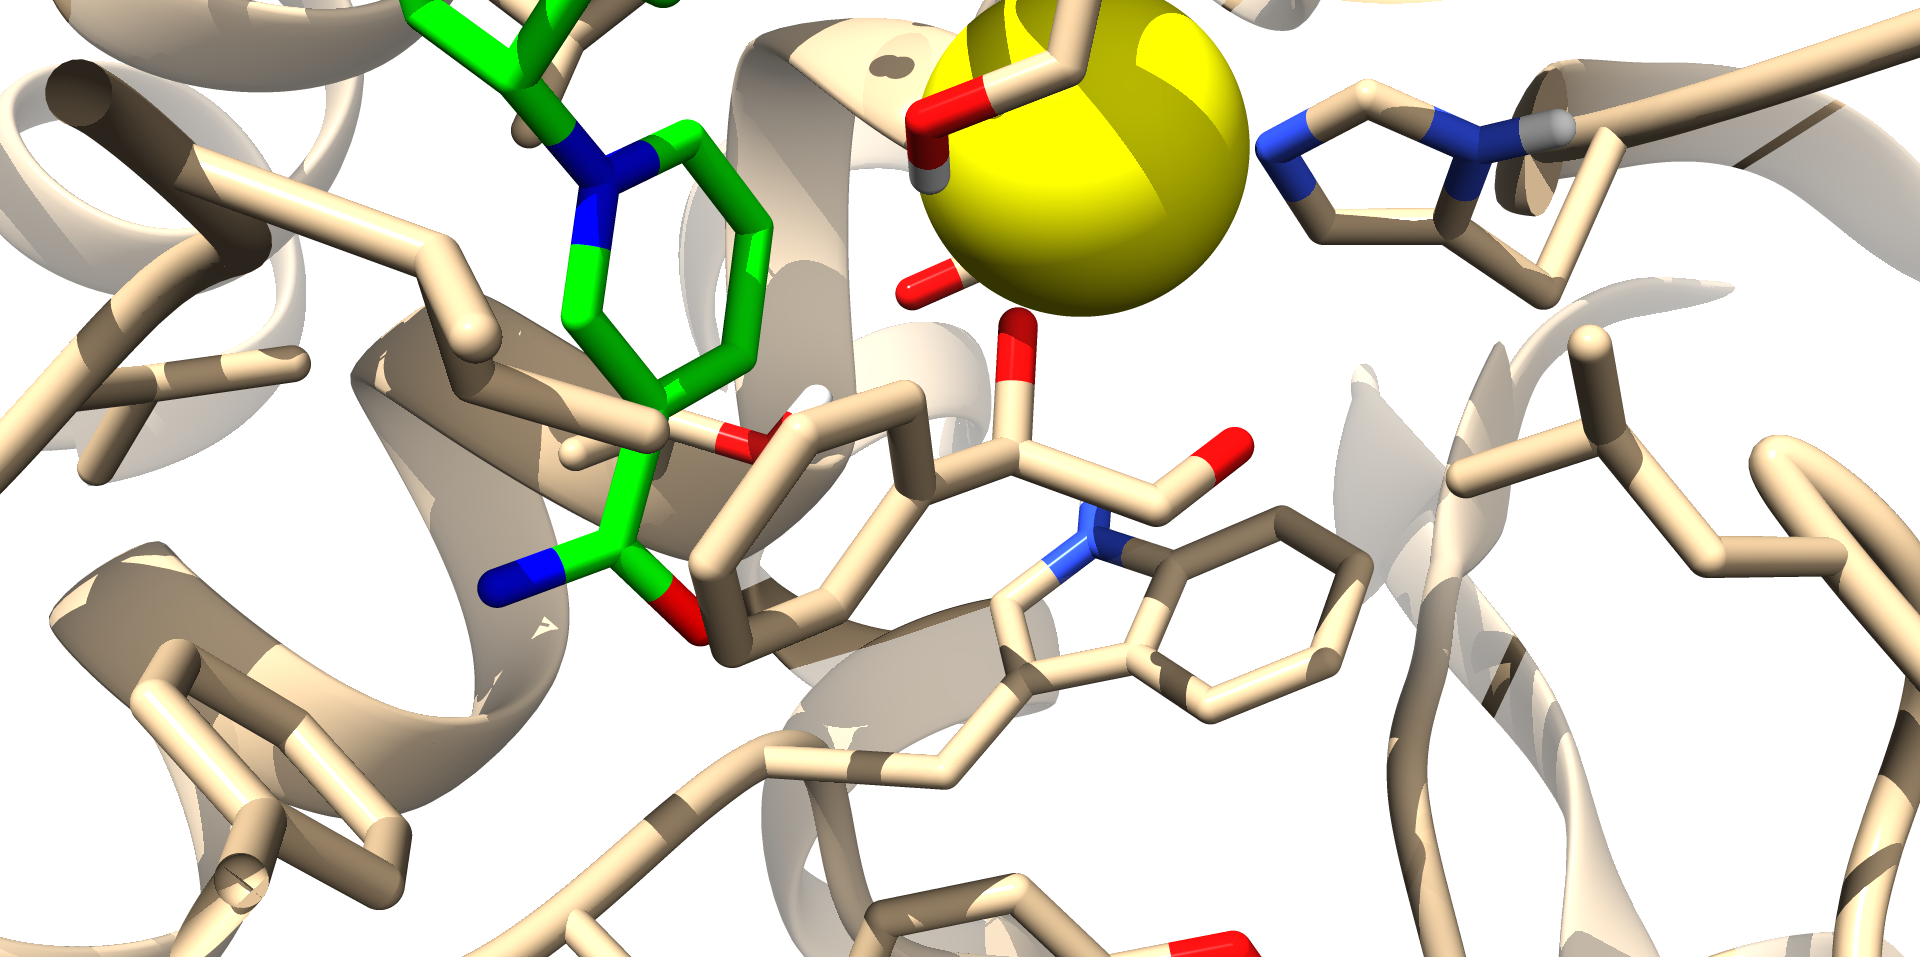
\includegraphics[width=\textwidth,keepaspectratio]{extra/diol-r.png}
		\caption{ADH-A active site with bound R-Phenylethanediol substrate}
		\label{fig:1.2}
	\end{subfigure}
	\caption{Different substrate binding orientations proposed for the two enantiomers of the Phenylethanediol substrate in ADH-A. Note the differences in distance between the nicotine-amide cofactor and the hydride donor.}
	\label{fig:1}
\end{figure}
%In both cases, the actual orientation stays the same, only the declaration in the CIP rule is changed due to the additional hydroxyl group.
The question is how this translates to the binding mode of the substrate in the active site, do both of them bind in a similar fashion, or are they showing completely different binding modes leading to the changes in catalytic activity.\\

\subsection{\rmfamily System preparation - PDB file and GRO file}
\label{sec:prepPDB}
To study the binding of the different substrate enantiomers, you are given a number of different systems that either contain the (R) or (S) enantiomer of one of the two enzymatic substrates phenylethanol and phenylethanediol.
Depending on your group, please investigate only one system each that has been assigned to you.
You will find the files in the archive \textit{course-material.tar.bz} that has been distributed to you before the course.
Please expand the archive in the project folder that you should have created according to section \ref{sec:create} under Day zero.
To due this, use the following command:

\begin{verbatim}
tar -xvf course-material.tar.bz
\end{verbatim}

These files will contain everything you will need to prepare the system with GROMACS.
You can explore them using commands like \textit{less} to open the files and see what they contain.
Go now to the folder indicated for your group, remember that you can see all folders and files using commands like:

\begin{verbatim}ll\end{verbatim}

In your group folder, navigate to the folder named \textit{0-pdb}.
It contains the PDB structure of your enzyme system, together with the substrate and co-factor bound in the active site.
You can visualize it if you want on your own computer using tools like VMD or PyMOL.
To continue with the preparation, you will need to copy the PDB structure to the next folder, \textit{1-topo}.
Do this the following way:

\begin{verbatim}
cp *.pdb ../1-topo 
\end{verbatim}
and then enter the directory with the command:

\begin{verbatim}
cd ../1-topo 
\end{verbatim}

Here, you will find in addition to your PDB file a folder containing the information for the program on how to prepare a structure to be simulated using the CHARMM36 force field.
Those files have been modified to include the substrates under study, as well as the zinc ions found in the enzyme and a special cysteine residue coordinating the zinc.
Before you can continue, you will now need to load the commands needed to run the GROMACS suite of programs on the supercomputer.
To do this, type the following:

\begin{verbatim}
module load gromacs/5.1.2
\end{verbatim}

You will have to remember to type this part every time you want to use GROMACS after you logged into the cluster.

Now, we are at the point that we can actually generate the first structure that GROMACS will know how to use.
Therefor, now type:

\begin{verbatim}
gmx_mpi pdb2gmx -f protein.pdb -o start.gro -ignh -ss -water 
tip3p -ff charmm36-jun2015
\end{verbatim}

This command will generate a new structure file containing all the residues in the internal GROMACS format, while also adding hydrogens to all atoms.
The command \textit{-ignh} first removes all protons, and then adds them back on, a useful way to get around a number of inconsistent naming schemes that exist for the protons encountered in a protein.
The other commands simply ask the program to use a certain PDB file (\textit{-f protein.pdb}), produce a certain output file (\textit{-o start.gro}) and allow the manual checking for the creation of disulfide bridges (\textit{-ss}).
It is important that you let the program create those for you, as they are needed for the overall stability of the system.

Now you are good on the way of preparing the system for use.
The next step is to adjust the total size of the system for the simulation, to allow for a buffer zone between the protein itself and the simulation boundaries.
The way we are going to simulate the behaviour is going to be under Periodic Boundary Conditions (PBC), where the system is going to be virtually replicated along all the simulations axis.
This allows the calculation of long range electrostatic effects and makes it possible for the solvent to freely move around, without the imposed structures of a hard border on any edge.
For more information about this and the way the effects are calculated, we can give you access to some articles that talk about both the mechanics and implications that this kind of calculation implies \cite{PBCAND,PME,SPME}.
To prepare the system for the PBC calculation, copy the files generated in the first folder to the next one, \textit{2-box}.
To do this, use the following command in the folder \textit{1-topo}:


\begin{verbatim}
cp start.gro *top *itp ../2-box
\end{verbatim}
and also enter the second folder

\begin{verbatim}
cd ../2-box
\end{verbatim}

The reason for following this procedure of several folders and copying the results from on into the next is that it will make it possible to revert mistakes at any step by simply copying the state of the files from the previous folder over the new one.
in this folder, the next command will adjust the size of the simulation and set the type of replicated structure from different shapes.
In general, it is prudent to find the shape of system that best fits to the protein being studied, to avoid an unnecessary amount of water that needs to be simulated.
You can think about having a ling stick in a cube, where most of the space around the actual interesting part (the stick) will be empty, or inside an elongated box, leaving less empty space.
In our case, the optimal box type has already been established as triclinic, so you do not have to do the testing yourself, but you are welcome to try at a later time to see if the system really will have the least amount of water molecules or not.
Now, to set the box type, do the following:

\begin{verbatim}
gmx_mpi editconf -f start.gro -o box.gro -bt triclinic -d 1.5 -c 
\end{verbatim}

The results of this command are that our simulation box is now centered on the solute (our protein), with a triclinic box around it and a distance of at least 1.5 nm to each side of the box edges.
The next step will now be covered in the following section of solvating and neutralising the system.
Before we go there, just make sure that you copy the files again to the next folder, using this command:

\begin{verbatim}
cp box.gro *itp *top ../3-solv
\end{verbatim}
and move yourself to this folder, too:

\begin{verbatim}
cd ../3-solv
\end{verbatim}


\subsection{\rmfamily System preparation - Solvation and ionisation}
\label{sec:solv}

We now have a minimal system done that we could use to run simulations on, but they would not be in a solvent but in gas phase.
To change this, we now have to instruct GROMACS to replace the empty space around the protein with our solvent of choice, here it will be water, and to be exact the TIP3P water model.
There are a large number of those models available that have different uses.
Our choice to use TIP3P is simply because it is the recommended model for use with the CHARMM36 force field we decided to employ for our calculations, so we are going to stick with it.
To solvate the system, use this command:

\begin{verbatim}
gmx_mpi solvate -cp box.gro -o solv.gro -cs spc216 -p topol.top
\end{verbatim}

This will use our previously prepared box (\textit{-cp box.gro}) together with an appropriate three point water molecule structure (\textit{-cs spc216}, do not be confused that the name here says SPC, a different kind of three point water molecule. It mainly tells GROMACS to use a box of prepared three point waters and has no effect on the actual parameters used later.) to generate the solvate structure (\textit{-o solv.gro}).
After this you can again have a look at your system using a molecular graphics program, you should see that the protein is now encased in solvent.
The program will also print the maximum number of solvent molecules, useful if you want to check on your own if the chosen box type is actually the best choice.

Only one more thing is now needed before the first simulation can start, the right choice of buffer and the neutralisation of the system.
We can not get to deeply into the reasons here for why simulations under our chosen conditions need to be on a neutral system, but it can be said that it is related to the calculation of the electrostatic interactions.
For this, again first copy your last results to the next folder, followed by changing the directory there:

\begin{verbatim}
cp solv.gro *itp *top ../4-ion
cd ../4-ion
\end{verbatim}

This is the first time we let the program test the validity of our parameters and files, as we have to create a special file now, the run control file \textit{ion.tpr}.
The program itself will generate it from the input file \textit{ion.mdp} that you will find in this folder.
The file itself contains the following instructions:\\

{\ttfamily \lstinputlisting[breaklines]{extra/ion.mdp}}~

To create the file for the generation and placement of ions, any valid input for GROMACS will work.
Here we used a minimal set of instructions also later used for the minimization of the system, but any other (valid) input file will work.
To now create the new \textit{ion.tpr} file, run this command:


\begin{verbatim}
gmx_mpi grompp -f ion.mdp -c solv.gro -p topol.top -o ion.tpr
\end{verbatim}

What you now have is a binary file in the internal GROMACS format, the same that is used to run the subsequent calculations.
If you got any error during this step, it means that either you missed to copy some file, or that you made a mistake in an earlier step.
This can happen, as it is quite difficult to get the exact sequence of commands right and not end up with corrupted files.
Try to follow the steps again or check your notes to see what you did at which point.
The ions itself are placed by a different GROMACS routine that we are going to use next:


\begin{verbatim}
gmx_mpi genion -s ion.tpr -p topol.top -o ion.gro -pname NA 
-nname CL -conc 0.15 -neutral
\end{verbatim}

When asked to place the salt molecules, chose group 17, representing the solvent molecules \textit{SOL}.
This command looks quite complicated now, because we need to specify the types of ions (\textit{-pname NA} for positive sodium ion and \textit{-nname CL} for negative chloride), as well as the final concentration of 0.15 mM (\textit{-conc 0.15}) and that we desire to have a neutral system in the end (\textit{-neutral}).
If this command now runs without an issue, the system is prepared for running the simulations, as it now contains all needed components.
You can copy the new files to the minimization folder, to prepare for the next step, and move there yourself:

\begin{verbatim}
cp ion.gro *itp *top ../5-minim
cd ../5-minim
\end{verbatim}~


\subsection{\rmfamily Protein minimization}

The next logical step on the way to simulate the protein is now to allow the atoms in the system to adopt an energetically optimal configuration for the chosen parameter set.
This process is called minimization and aims to remove all the strain that might be present in a crystal structure or complex.
Those strains could have been included due to a number of factors, including low resolution in the crystal and resulting suboptimal placement of sidechains, differences in crystal parameter sets and those used for the simulation, placement of hydrogen atoms where they do not belong, ...
To deal with this, we minimize now according to a steepest decent algorithm.
There are other choices available that have different usage depending on the problem, but we will stick to the more simple one for now.
The file you are going to use is \textit{min.mdp}:\\

{\ttfamily \lstinputlisting[breaklines]{extra/min.mdp}}~

The options in the file are telling you now exactly how the program is instructed to proceed with the minimization of the structure.
We are now telling it to use the steepest decent minimizer (\textit{integrator steep}) and give it some further instructions on how the minimization should proceed and when the program should stop.
The following command creates the input file \textit{min.tpr}:

\begin{verbatim}
gmx_mpi grompp -f min.mdp -c ion.gro -p topol.top -o min.tpr
\end{verbatim}

Now you have in your hands the file you need to start the first calculation to minimize the energy of the system.
But you should not do this right away, as it would cause the program to be started on the same part of the cluster that all user use for logging in and viewing files, and would actually be stopped after a short time due to this.

The simulations should now be submitted to the actual computation nodes of the cluster, to be simulated there instead.
There are two main ways how to do this, either by writing a short script that takes care of the submission and running of the program, or by asking for interactive access to a computation node.
In the case of our minimization and equilibration will use the interactive pathway, as it will allow us to directly interact with the program.
Type the following into the command line on the cluster:

\begin{verbatim}
interactive -A snic2017-5-49 -t 02:00:00 -n 16
\end{verbatim}

This will ask for access to sixteen computation cores of one node of the cluster for 2 hours.
It may take a while until the access is granted, so be patient.
Once you see that you are in a new window, you can start loading the software again (\textit{module load gromacs/5.1.2}) and then run the minimization by using the command:

\begin{verbatim}
mpprun -n 16 gmx_mpi mdrun -deffnm min 
\end{verbatim}

The software will now start to calculate and will update you periodically about the progress.
Once it is done, you can close the connection to the computation node using \textit{exit}.
%Once it is done, you can close the connection to the computation node using \textit{Shift-Control-D}.

\subsection{\rmfamily Protein heating and equilibration}

The last two steps of todays tasks are concerned with the final heating up of the protein and the equilibration that would proceed the long time scale simulations.
They follow in the main concept the steps we have already undertaken to minimize the system, with equivalent commands to be executed for each.
First, you will need to again copy the files you got from the minimization to the next folder, followed by changing the directory to the new place:

\begin{verbatim}
cp min.gro *itp *top  ../6-nvt
cd ../6-nvt
\end{verbatim}

In this folder you will find a new input file, \textit{nvt.mdp}, that will govern the relaxation and heating of the protein now using the constant particle (\textit{N}), volume (\textit{V}) and temperature (\textit{T}) ensemble.\\

{\ttfamily \lstinputlisting[breaklines]{extra/nvt.mdp}}~

If you are interested, you can again look up the meaning of the different commands, we are only going to cover a few of them here.
Most important is now the choice of the integrator (\textit{integrator md}), telling the program to propagate velocities according to newtons equations of motion, the number of steps (\textit{nsteps 100000}) telling the program how long the simulation should be, and the timestep for each calculation step (\textit{dt 0.001}), that tells us that every step is 1 fs in time, leading to a total simulation time of 100 ps.
Using this file, you can now create again the real input file needed for the program to perform the calculation:

\begin{verbatim}
gmx_mpi grompp -f nvt.mdp -c min.gro -p topol.top -o nvt.tpr -n 
index.ndx
\end{verbatim}

When this is done, again ask for the interactive node and start the calculation when it has started:

\begin{verbatim}
interactive -A snic2017-5-49 -t 02:00:00 -n 16
module load gromacs/5.1.2
mpprun -n 16 gmx_mpi mdrun -deffnm nvt
\end{verbatim}

Repeat those steps for the final part of the calculation in the folder \textit{7-npt} to finish the task for today.
If you are interested, you can then have a look at the structures generated from the minimization, heating and equilibration, to see where molecules move.
You can do this by following the instructions later in the manual in section \ref{sec:dataanalysis}, just replacing the names of the files with those you obtained from the calculations here.
But keep in mind that the time scales chosen for this tutorial are very short compared to the time it usually takes to fully simulate a system.
This is why we are going to investigate already finished simulations tomorrow to give us some better feeling on what might happen during this kind of calculation.

\begin{verbatim}
gmx_mpi grompp -f npt.mdp -c nvt.gro -p topol.top -o npt.tpr -n 
index.ndx
interactive -A snic2017-5-49 -t 02:00:00 -n 16
module load gromacs/5.1.2
mpprun -n 16 gmx_mpi mdrun -deffnm npt
\end{verbatim}


\clearpage
\section{\rmfamily Day 2}
\subsection{\rmfamily Data analysis - Mirror images and artefacts}
\label{sec:dataanalysis}
Hello again to the second part of this tutorial.
During this part, your groups will again be distributed to work on different parts so that each group will analyse its own set of data from simulations that have been done previously by a student.
To start, I would like you to load the visualization software VMD (\textit{module load vmd/1.9.1}) that will be needed later for the analysis.
For a manual of this program, I can point you to a tutorial (https://www-s.ks.uiuc.edu/Training/SumSchool/ materials/sources/tutorials/01-vmd-tutorial/html/node2.html) for help.  
Make sure that you set up the connection to the cluster using X forwarding, as shown below in section \ref{sec:xforward}.
Then, you should enter the directory belonging to your group at the following location \textit{/proj/alcohol\_dehydrogenase\_a/}.
The files have been deposited there because they would have been too large to distribute them.
In this folder you will find a number of files when using e.g. \textit{ll}, among them a structure file \textit{npt.gro}, a run input \textit{md.tpr} and a trajectory file \textit{md-small.trr} containing the coordinates of the system at different time points.
The first thing you can try is loading the files directly into VMD using the following command:

\begin{verbatim}
vmd npt.gro md-small.trr
\end{verbatim}

Be prepared to wait a while, it will take time to load everything into the program.
When done loading, you might see some strange things, with molecules being broken in the middle or jumping around.
This is caused by the fact that the simulations were done under periodic boundary conditions and that the molecules move through the minimum unit described, passing the border on one side and reappearing on the next.
If we want to analyse the system, we first need to get rid of this problem by telling the program to reconstitute the system in each saved step.
To do this, we will again use GROMACS on the full trajectory file you have, \textit{md.trr}, the other file was kept smaller to allow fast visualisation.
So, load GROMACS again, and then use this command

\begin{verbatim}
gmx_mpi trjconv -f md.trr -s md.tpr -n index.ndx -o md-noPBC.trr 
-pbc mol -ur tric -center
\end{verbatim}

Now you should have a new trajectory file with the corrected coordinate information.
If you want to check this, I recommended you to run the same command with a different file name for \textit{-o md-noPBC.trr} to get a new file, and with the added option of \textit{-dt 500}.
Then you can load this new file again into vmd, together with the \textit{npt.gro} file.\\

\subsection{\rmfamily Data analysis - RMSD}

Now that the files are ready for the further analysis, the first things to investigate are the overall stability of our system, how much it moves away from the set of coordinates saved in the crystal, and how much fluctuation is observed during the time of our simulation.
This is achieved by calculating the Root mean squared deviation (RMSD) of the system.
What this means is that our program will first try to fit our system to the closest possible distance to all atoms in a set we want to investigate, and will then calculate the remaining distances for all atoms.
To actually have a look at all the different interesting parts (whole protein, active site, cofactor, substrate), we will have to perform several of those calculations after another.
The first calculation will be on the whole system, after performing the fitting to the backbone atom positions

\begin{verbatim}
gmx_mpi rms -s md.tpr -f md-noPBC.trr -n index.ndx -o 
rmsd-protein.xvg -tu ns
\end{verbatim}

When asked for the reference structure (first question), chose \textit{4} (Protein Backbone), while for the question about the actual data set (the second question) chose \textit{1} (Protein).
This will now perform the calculation on all structures, and when finished write out a single file \textit{rmsd-protein.xvg}.
This is just a normal plot that can be visualized with Linux tools like xmgrace.
The program is already loaded by default on the cluster, and you can have a look at the plot using \textit{xmgrace rmsd-protein.xvg}.
In there, you will also be able to save this plot as a graphic by first choosing \textit{Print options} under the \textit{File} menu, selecting \textit{Print to file} and then choosing \textit{Print}.
You can also change the print option to print to other file types, such as pdf or ps.
As default this will create a postscript file that you can open in vector graphics programs such as Inkscape.

Repeat this one for the RMSD calculations of the protein backbone fitted to the protein backbone, the substrate (the selection called \textit{OPE} or \textit{OPD}, depending on if you are investigating the alcohol or the diol substrate), the cofactor \textit{NAD} and the metal ions \textit{ZD4}.
For each of the calculations you should use a new file name for the data file you are creating.
What can you say now about the overall stability of the protein and its ligands?
Are there any surprising or concerning behaviours?\\

\subsection{\rmfamily Data analysis - Distance measurements}

To continue the data analysis, we will now investigate the actual distances between the reacting atoms in our system, together with the coordination of the substrate to the metal.
To be able to measure this kind of interactions, we could either try to look at them by hand in a graphics program, or we could let one of the GROMACS program do the analysis for us.
We will go with the analysis program \textit{gmx\_mpi distance}, as it will not only generate the measurements, but can also give us important information about the distribution of bond distances.
To be able to do so, we will first need to make GROMACS understand what we want to measure by telling it the atoms we are interested in.
This is done using the program \textit{gmx\_mpi make\_ndx}.
Here, a user can specify any group of atoms so it can be reused again later in a different program of the GROMACS package.
Your teachers actually used this program to prepare some of the input files needed for the calculations yesterday, namely the \textit{index.ndx} files.
Now, you are going to prepare a new set of those files, called \textit{measure.ndx}.
To do so, use the following command line in your current directory, \textit{DIOL|ALCOHOL/R|S/8-analysis}.

\begin{verbatim}
gmx_mpi make_ndx -f md.tpr -n index.ndx -o measure.ndx
\end{verbatim}

This will start the program from the already existing \textit{index.ndx} file to create the new file.
The usage of it seems quite complicated in the beginning, but with some time you will get the hang of it.
The first thing to remember is that you can always abort the current run of the program pressing \textit{Control C} and start again, if you by mistake delete an important group.
You can select and mix or combine groups using the binary operators \textit{!, \&, | (not, and, or) }, while typing \textit{h} followed by enter will display a help text.
Now, to do something like selecting two atoms for a distance measurements you can do the following, an example for the substrate Hydride and acceptor carbon on NAD$^+$.

\begin{verbatim}
14 & r 504 & a NC2
15 & a H13
23 | 24
name 25 DistHYD-NAD
\end{verbatim}

You can try to perform all of those assignments yourself for the following residues, or you can use the already prepared file \textit{measure2.ndx}.
The residues of interest are:
\begin{itemize}
\item{Zinc 502 (ZD4, center atom Z41)}
\item{Aspartate 153 (ASP, oxygens OD2 and if needed OD1)}
\item{Histidine 62 (HISD, nitrogen NE2)}
\item{Cysteine 38 (CYN, sulphur SG)}
\item{Substrate OPE or OPD (oxygen O14)\\}
\end{itemize}

Create the paring of each of those atoms with the center atom of the metal, and use those new groups for the calculations further on.
One thing that GROMACS does not tell you is that your residues are in chain B (the second number) of the structure.
IF you want, you can also prepare the group needed for the final calculation of the clustering, composed of residues \textit{38, 40, 62, 153, 269, 271, 281, 286, 294, 295, 502, 504, 505}.
Again, this group is also already created in the file \textit{measure2.ndx}.
Now you can perform the actual measurement, here shown the command my using my \textit{measure2.ndx} and the groups therin, for your own files you would need to adjust the numbers.

\begin{verbatim}
gmx_mpi distance -s md.tpr -f md-noPBC.trr -n measure2.ndx -oall 
distances.xvg -oh histogram.xvg -oallstat statistics.xvg -len 
0.3 -tol 3 -tu ns -select 23 24 25 26 27 28
\end{verbatim}

Now you will get a number of files containing different information about the distances during the calculation.
You can again visualize them using \textit{xmgrace}, but this time you will need to start the program first and then import the files so that all traces are plotted together.
Again, do you see any interesting, alarming occurrences?
What do they tell you about the stability of the active site and the substrate?\\


\subsection{\rmfamily Data analysis - Clustering of structures}

The final part of the tutorial will be the clustering of structures to see if there are any distinguishable populations of structures during the simulation,
 and to investigate how those might transition between each other.
We will again use one of the GROMACS tools build for this kind of analysis, \textit{gmx\_mpi cluster}.

\begin{verbatim}
gmx_mpi cluster -s md.tpr -f md-noPBC.trr -n measure2.ndx -dist 
-sz -ntr -cl 
\end{verbatim}

Again, if you want to find out what the options mean for the calculation, you can use the command \textit{gmx cluster -h} to print a comprehensive help text.
This can also be useful if you want to set up your own clustering calculations later.
When prompted by the program, select the group composing the active site (group \textit{active} in case of measure2.ndx, or the name you gave it) for the first selection, and the whole system (\textit{Group 0}) for the print out.
As those calculations will take a long time, and are intensive in terms of calculation power needed, it would be recommended to use the interactive computation nodes again as on Day 1.
Otherwise it might happen that the process gets terminated by the automatical control systems on Triolith.

In the end, you will receive a number of files again, that you can visualize in \textit{xmgrace} for the plots, or load into programs like VMD, PyMOL or Chimera in case of the PDB files.
What do you see?
Do the clusters show any strange behaviour of the active site?

\clearpage
\section{\rmfamily Day three}
\subsection{\rmfamily Synopsis}
You have now managed to both set up a new simulation almost from scratch (we ignored the boring parts of generating parameters for our ligands and preparing the force field to use them).
This would involve more complex calculations and some Quantum Chemistry simulations that are beyond the scope of this short tutorial.
If you want, you can use the extra time now to try your own simulation set up, based on what you saw during the first and second day.
You can for example try different positions of the substrate in the active site, to see if you can simulate the minimization of different binding modes.
Or you could try to do something similar on other proteins from the Protein Data Base (http://www.rcsb.org) if you are inclined to this.
Also, this is the time to ask any questions that you might have had during the lab and haven't had the chance for.

We hope that we could give you some insights into how protein simulations are performed with this small example.

\clearpage
\setcounter{section}{-1}
\section{\rmfamily Day zero}
\subsection{\rmfamily The Unix shell, connecting}
Most computational chemistry programs are run under a Unix or Linux environment, and the program GROMACS is no different in this aspect.
Those few lines here should give you some familiarity with the Unix shell and point you to places where you can find help (in general, Google is always the best friend).
We are going to work on a command line based connection to one of the supercomputers, Triolith.
This means that all our commands will be text based, and you should be able to copy most of them directly from this tutorial to the command line.
There are a few commands that you will have to keep in mind, such as \textit{ll} or \textit{ls}, listing the files of a directory, or \textit{cd}, changing the directory either to one found below the current one, one above when prefixed like \textit{cd ../} or to the home directory when used without any targets.
Text files can be viewed with editors such as nano, emacs or vim.
I recommend you to try to use some of the commands first before going to the lab, and also trying out some of the editors to see which one works best for you.
More help can also be found in this Tutorial (http://www.ee.surrey.ac.uk/Teaching/Unix/).

To connect to the Triolith cluster, you will have to use one of the tools available on the computers available.
If you use PuTTY, open the program, and chose \textit{triolith.nsc.liu.se} as the host name.
If prompted, accept the server key, and continue by giving the username and password you should have received from NSC.
You will likely be asked to provide another password, do this and then continue with the rest of the tutorial.

If you want to transfer files you can use WinSCP, after connecting in the same manner as with PuTTY.
If this is not working, please ask a lab assistant for help.\\

\subsection{\rmfamily X Forwarding}
\label{sec:xforward}
To be able to use some of the graphic interfaces on the cluster, you will have to enable an option called X Forwarding.
This basically means that you want graphical output from the cluster to be sent to the current machine.
In case of PuTTY, after setting up the general connection, scroll down on the left sidebar and go to the section \textit{Connection > SSH > X11}.
There, select the option and you are good to go.
In case of Mac or Linux, simply connect like this:

\begin{verbatim}
ssh -X yourname@triolith.nsc.liu.se
\end{verbatim}

Then you will also be able to forward the graphical output.\\


\subsection{\rmfamily Creating and removing folders}
\label{sec:create}
The first thing to prepare for our future work are the directories we are going to need.
For this part it is important to know that the space on the supercomputer is limited for each user, so you will not be able to perform all the task within your own home folder.
Instead, you will work in the directory created for the course that has larger storage capacity.


To make this easier, we will first create something called a link, that will make it possible to easily access the directory.
Enter the following command:

\begin{verbatim}
cd /proj/alcohol_dehydrogenase_a/
\end{verbatim}

In this directory, you can now create your own user directory by typing the command below

\begin{verbatim}
mkdir $USER 
\end{verbatim}

You should do all your work in your own directory like this.
This will both make sure that you are not running out of space, and ensure that you have a central space for your files only.\\


\subsection{\rmfamily Archives}
The data for this course will always be given to you, or be available on the cluster as an archive called \textit{tarball}.
The first archive, \textit{for\_students.tar.gz}, contains all the files needed for you to perform the task on Day 1 of the lab, while the files for the second task will be provided separately.
To set up your directories, you will need to unpack the first archive in your work folder that you created in \ref{sec:create}.
For this, first copy the files there using WinSCP (or any scp client of your choice).
Get the full length path of the directory by using \textit{pwd} while you are there, and copy this to the SCP client.
Once the file has been transferred, unpack it using the following command:

\begin{verbatim}
tar xf for_students.tar.gz
\end{verbatim}

Now all the files are present in the directories below.\\

\subsection{\rmfamily Copying of files and folders}
If you want to copy files while you are on the cluster, you can do this by using the \textit{cp} command.
The general syntax is that you can give a set of files to copy as the first n arguments for the command, followed by a single destination.
If you have decided to copy several files at once, the destination has to be a directory.
If you want to copy directories, you can use \textit{cp -r}, with the same limitations for the targets and the destination.
You can also use more advanced commands such as \textit{rsync}, but as they are more complicated this is not recommended if you are not already familiar with them.\\


\bibliographystyle{acm}
\footnotesize
\bibliography{references.bib}

\end{document}
